\section{Jadwal Pelaksanaan}

Berikut adalah rencana jadwal pengerjaan tugas akhir:

\begin{figure}[ht]
    \centering
    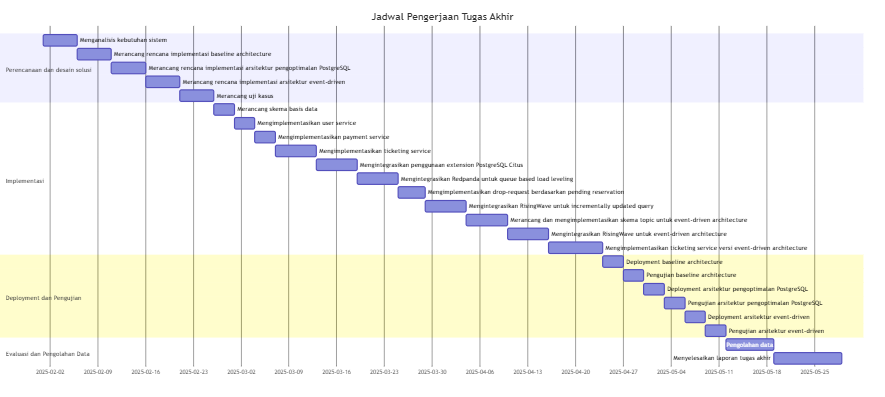
\includegraphics[width=1\textwidth]{resources/schedule/schedule.png}
    \caption{Jadwal Pelaksanaan}
    \label{fig:jadwal pelaksanaan}
\end{figure}

Secara umum, proses pengerjaan terbagi menjadi empat tahap, yaitu:

\begin{enumerate}
    \item Tahap perencanaan yang meliputi penentuan kebutuhan, perancangan implementasi, dan perancangan uji kasus.
    \item Tahap implementasi yang meliputi implementasi untuk tiga arsitektur, yaitu arsitektur dasar acuan, arsitektur yang mengoptimalkan PostgreSQL, dan arsitektur \textit{event-driven}.
    \item Tahap \textit{deployment} dan pengujian setiap arsitektur.
    \item Tahap penyelesaian yang meliputi pengolahan data dan menyelesaikan sisa pekerjaan laporan tugas akhir.
\end{enumerate}